\documentclass{../common/SCNU_Experimental_Report}

% 填写报告头信息
\studentname{汤承洲}
\studentid{20233902058}
\major{电子信息工程}
\class{23级2班}
\coursename{控制工程}
\projectname{MATLAB基本操作 MATLAB编程 MATLAB底层图形控制}
\verify
\experimentdate{2026年5月19日}
\teacher{熊爱民}

\begin{document}
\maketitle

\section{实验目的}
\begin{enumerate}
    \item \textbf{实验一 MATLAB基本操作：}熟悉MATLAB实验环境，练习MATLAB命令与m文件基本操作；利用MATLAB编写程序进行矩阵运算、图形绘制、数据处理等；熟悉矩阵相关的基本函数和命令；熟练使用帮助系统。
    \item \textbf{实验二 MATLAB编程：}熟悉MATLAB程序设计的基本方法；掌握for、while、switch-case、if控制结构；掌握MATLAB函数的编写方法。
    \item \textbf{实验三 MATLAB底层图形控制：}理解MATLAB中的句柄概念；利用MATLAB命令获取句柄及对图形目标进行属性设置；掌握gcf、gca、get、set等句柄操作函数的使用。
\end{enumerate}

\section{实验原理}
\subsection{MATLAB基本操作原理}
MATLAB是一种为数值计算、数据分析和图形显示服务的交互式环境。MATLAB有三种主要窗口：命令窗口（Command Window）用于交互式执行命令；m文件编辑窗口（Edit Window）用于编辑脚本和函数；图形窗口（Figure Window）用于显示图形结果。Simulink另有独立的模型编辑窗口。用户可以在命令窗口中直接输入命令立即执行，也可以将一系列命令写入m文件后批量运行。

矩阵是MATLAB中最基本的数据类型，所有数值计算均基于矩阵运算。MATLAB提供了丰富的矩阵操作函数，包括矩阵乘法、求逆、特征值分解、行列式计算等。

\subsection{MATLAB编程原理}
MATLAB支持标准的程序控制结构：
\begin{itemize}
    \item \textbf{for循环：}按照预设的迭代次数重复执行代码块
    \item \textbf{while循环：}当条件满足时重复执行代码块
    \item \textbf{if/elseif/else：}根据条件分支执行不同代码
    \item \textbf{switch/case：}多路分支选择结构
\end{itemize}

MATLAB函数通过\texttt{function}关键字定义，格式为\texttt{function[输出变量列表]=fun\_name(输入变量列表)}。函数文件需以函数名命名（\texttt{fun\_name.m}），并放置在MATLAB搜索路径中以便调用。

\subsection{MATLAB图形句柄原理}
MATLAB为所创建的每一个图形对象分配一个句柄（Handle），类似于指针。用户可以通过函数获取对象句柄并对其进行属性控制。图形对象具有严格的树形继承关系：

\begin{center}
根屏幕（Root，句柄值0）$\rightarrow$ 图形窗口（Figure，整数句柄）$\rightarrow$ 轴（Axes）$\rightarrow$ 线/面/字/块/像
\end{center}

关键句柄操作函数：
\begin{itemize}
    \item \texttt{get(handle)}：获取图形对象的属性值
    \item \texttt{set(handle, property, value)}：设置图形对象的属性
    \item \texttt{gcf}（Get Current Figure）：返回当前图形窗口的句柄
    \item \texttt{gca}（Get Current Axes）：返回当前坐标轴的句柄
    \item \texttt{handle.Children}：访问当前对象的所有子对象
\end{itemize}

\section{实验内容}
\subsection{实验一：MATLAB基本操作}

\subsubsection{Task 01：矩阵输入与乘法运算}
输入两个矩阵A（$5\times4$）和B（$4\times6$，含复数元素），计算乘积矩阵C = A $\times$ B，并提取C右下角的$2\times3$子矩阵赋给D，完成后查看MATLAB工作空间的占用情况。

\begin{lstlisting}[language=Matlab]
A = [1, 2, 3, 3; 2, 3, 5, 7; 1, 3, 5, 7; 3, 2, 3, 9; 1, 8, 9, 4];
B = [1+4i, 4, 3, 6, 7, 8; 2, 3, 3, 5, 5, 4+2i;
     2, 6+7i, 5, 3, 4, 2; 1, 8, 9, 5, 4, 3];
C = A * B;
D = C(end-1:end, end-2:end);
whos;
\end{lstlisting}

\textbf{实验结果：}矩阵乘法成功执行，C为$5\times6$复矩阵，D为C右下角$2\times3$子矩阵。工作空间显示：A（5x4 double）、B（4x6 complex double）、C（5x6 complex double）、D（2x3 complex double），四个变量共占用约1120字节。

\subsubsection{Task 02：绘制 $y = \sin(1/t)$ 曲线}
选择合适的步距绘制$y = \sin(1/t)$，其中$t \in (-1, 1)$。为避免$t=0$处的奇点，将区间分为$(-1, -0.001)$和$(0.001, 1)$两段，各取2048个采样点，在0附近采用更密集的采样以捕捉高频振荡。

\begin{figure}[H]
    \centering
    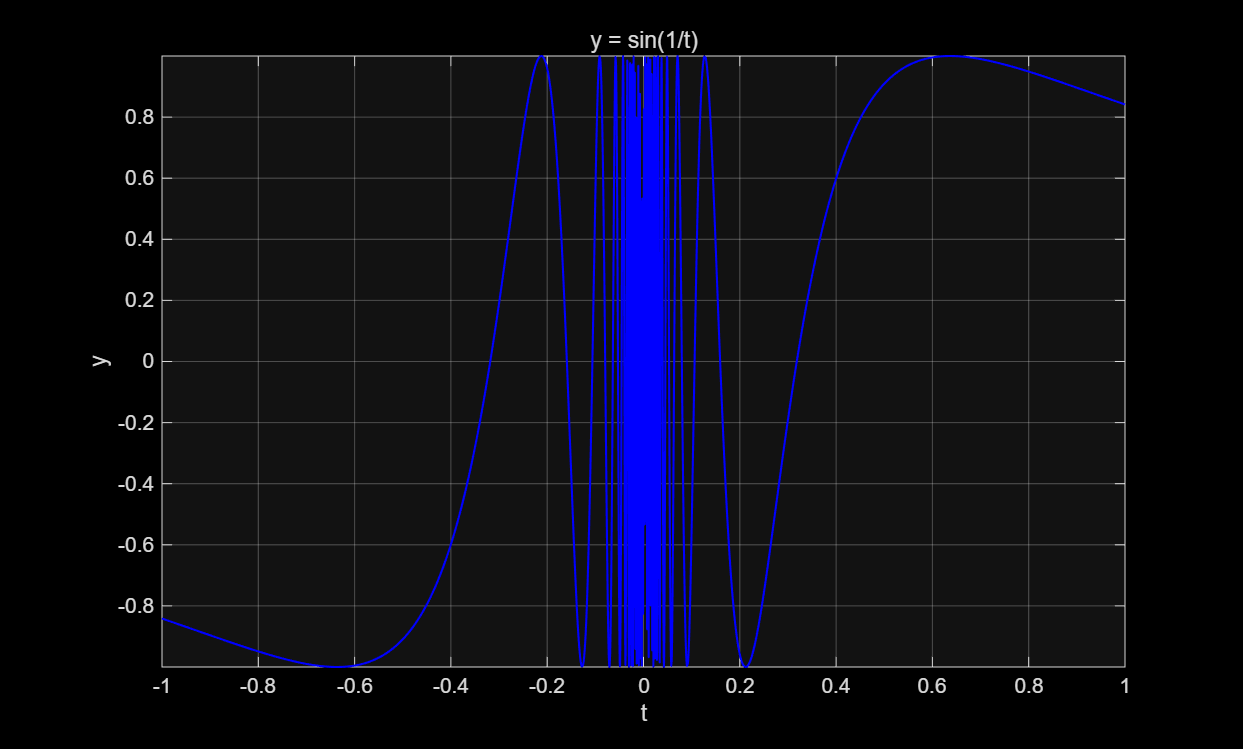
\includegraphics[width=0.75\textwidth]{./figures/Ex1_Task02_Figure_01.png}
    \caption{实验一 Task 02：$y = \sin(1/t)$ 曲线图}
    \label{fig:ex1_task2}
\end{figure}

\textbf{实验结果：}函数在$t \to 0$时振荡频率趋于无穷大，两端振荡逐渐减缓。曲线在原点附近呈现密集的高频振荡特征。

\subsubsection{Task 03：矩阵分析}
对给定的四个$4\times4$矩阵A、B、C、D分别求取行列式、秩、特征多项式、范数、特征值、特征向量和逆矩阵（若存在）。

\begin{table}[H]
    \centering
    \caption{实验一 Task 03：矩阵分析结果汇总}
    \label{tab:ex1_task3}
    \small
    \begin{tabular}{cccccc}
        \toprule
        矩阵 & 行列式 & 秩 & 2-范数 & 特征值个数 & 是否可逆 \\
        \midrule
        A & 432221 & 4 & 103.72 & 4（全实根） & 是 \\
        B & 1 & 4 & 30.29 & 4（全实根） & 是 \\
        C & $\approx$0（$6.2\times10^{-30}$）& 2 & 38.62 & 2非零+2近零 & 否（奇异） \\
        D & 595 & 4 & 16.70 & 2实根+2复共轭 & 是 \\
        \bottomrule
    \end{tabular}
\end{table}

\textbf{实验结果：}矩阵C为奇异矩阵，行列式近似为零，秩仅为2，存在2个接近零的特征值（$\approx -2.9\times10^{-15}$和$\approx -5.7\times10^{-16}$），因此不可求逆。其余三个矩阵均为满秩可逆矩阵。

\subsubsection{Task 04：求解线性方程组}
使用MATLAB反斜杠运算符（\texttt{\textbackslash}）求解两个线性方程组$AX = B$，并通过残差范数$\|AX - B\|_F$验证解的准确性。

\begin{table}[H]
    \centering
    \caption{实验一 Task 04：线性方程组求解结果}
    \label{tab:ex1_task4}
    \small
    \begin{tabular}{ccc}
        \toprule
        问题 & 解向量X & 验证残差 \\
        \midrule
        (a) & $[0.4979, 0.1445, 0.0629, -0.0813]^T$ & $5.44\times10^{-16}$ \\
        (b) & 两列解向量（$4\times2$矩阵） & $2.06\times10^{-15}$ \\
        \bottomrule
    \end{tabular}
\end{table}

\textbf{实验结果：}两个问题的残差均在机器精度范围内（$< 10^{-14}$），解精确满足原方程。

\subsubsection{Task 05：矩阵初始化与操作}
(1)(2)(3) 分别使用\texttt{ones(10)}、\texttt{zeros(10)}、\texttt{diag(1:10)}初始化特殊矩阵。\\
(4) 输入$A=[7,1,5; 2,5,6; 3,1,5]$和$B=[1,1,1; 2,2,2; 3,3,3]$，练习矩阵索引（\texttt{A(2,3)}、\texttt{A(:,2)}、\texttt{A(3,:)}、\texttt{A(:,1:2:3)}）、赋值（\texttt{A(3,:)=B(2,:)}）以及矩阵运算（\texttt{*}, \texttt{.*}, \texttt{\^2}, \texttt{/}, \texttt{./}）。

\textbf{实验结果：}
\begin{itemize}
    \item \texttt{A(2,3) = 6}（访问第2行第3列元素）
    \item \texttt{A(:,2) = [1; 5; 1]}（访问第2列所有行）
    \item \texttt{A(3,:) = [3, 1, 5]}（访问第3行所有列）
    \item \texttt{A(:,1:2:3)}返回第1列和第3列（步长为2）
    \item 矩阵乘法\texttt{A*B}得到$3\times3$结果矩阵，逐元素乘法\texttt{A.*B}维度相同但元素为对应乘积
    \item 矩阵右除\texttt{B/A}（等价于$BA^{-1}$）与逐元素右除\texttt{B./A}结果截然不同
\end{itemize}

\subsubsection{Task 06：同一坐标系绘制曲线}
在同一坐标系中绘制$y = \cos(t-0.5)$（红色实线）和$y = \sin(t-0.5)$（蓝色虚线），$t \in [0, 2\pi]$，使用不同颜色和线型区分，并设置\texttt{axis equal}控制坐标轴比例。

\begin{figure}[H]
    \centering
    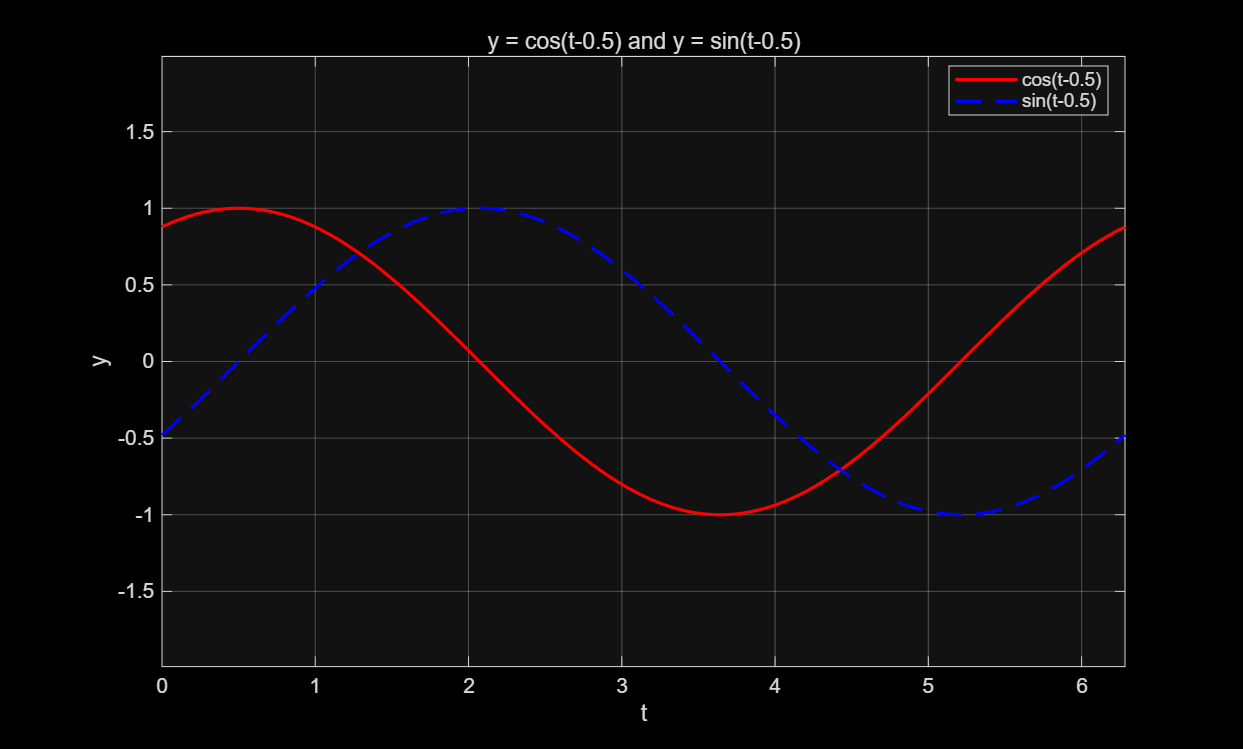
\includegraphics[width=0.75\textwidth]{./figures/Ex1_Task06_Figure_01.png}
    \caption{实验一 Task 06：$y = \cos(t-0.5)$与$y = \sin(t-0.5)$同一坐标系绘制}
    \label{fig:ex1_task6}
\end{figure}

\subsection{实验二：MATLAB编程}

\subsubsection{Task 01：求$K = \sum_{i=0}^{63} 2^i$}
分别使用for循环、while循环和向量化（无循环）方法计算$K = 2^0 + 2^1 + \cdots + 2^{63}$。理论值：$K = 2^{64} - 1 = 18446744073709551615$。

\textbf{实验结果：}三种方法均得到完全相同的结果：
\begin{itemize}
    \item for循环结果：18446744073709551615
    \item while循环结果：18446744073709551615
    \item 向量化结果（$2^{64} - 1$）：18446744073709551615
\end{itemize}
使用\texttt{uint64}类型确保64位整数不溢出。向量化方法利用等比数列求和公式$S_n = (r^{n} - 1)/(r - 1)$将O(n)复杂度降为O(1)。

\subsubsection{\texorpdfstring{Task 02: 求$1+2+\cdots+n < 10000$的最大$n$}{Task 02: 求1+2+...+n < 10000的最大n}}
使用while循环逐渐累加，当累加和即将超过10000时停止。

\textbf{实验结果：}
\begin{itemize}
    \item 最大$n = 140$
    \item $1+2+\cdots+140 = 9870 < 10000$
    \item $1+2+\cdots+141 = 10011 \geq 10000$（超出阈值）
\end{itemize}
验证：由等差数列求和公式$S = n(n+1)/2$，$140 \times 141 / 2 = 9870$，结果一致。

\subsubsection{Task 03：分段函数$f(x)$的实现与测试}
编写函数文件\texttt{ff.m}实现以下分段函数（$D=1$，$h=10$）：
\[
y = f(x) = \begin{cases}
h, & x > D \\
\frac{h}{D}x, & |x| \leq D \\
-h, & x < -D
\end{cases}
\]

\begin{table}[H]
    \centering
    \caption{实验二 Task 03：分段函数测试结果}
    \label{tab:ex2_task3}
    \small
    \begin{tabular}{cccc}
        \toprule
        $x$ & $f(x)$ & 期望值 & 所在区间 \\
        \midrule
        $-1.5$ & $-10$ & $-10$ & $x < -D$（下饱和区） \\
        $0.5$  & $5$    & $5$    & $|x| \leq D$（线性区） \\
        $5$    & $10$   & $10$   & $x > D$（上饱和区） \\
        \bottomrule
    \end{tabular}
\end{table}

\textbf{实验结果：}三个测试点均正确，分段函数实现了典型的饱和线性特性（限幅放大器模型）。

\subsection{实验三：MATLAB底层图形控制}

\subsubsection{Task 01：基本图形句柄获取}
创建$y = \sin(t)$（Figure 1）和$y_1 = \cos(t)$（Figure 10）两个图形窗口，分别获取根屏幕句柄（\texttt{get(0)}）、两个图形窗口句柄（\texttt{get(1)}和\texttt{get(10)}），查看其属性。

\begin{figure}[H]
    \centering
    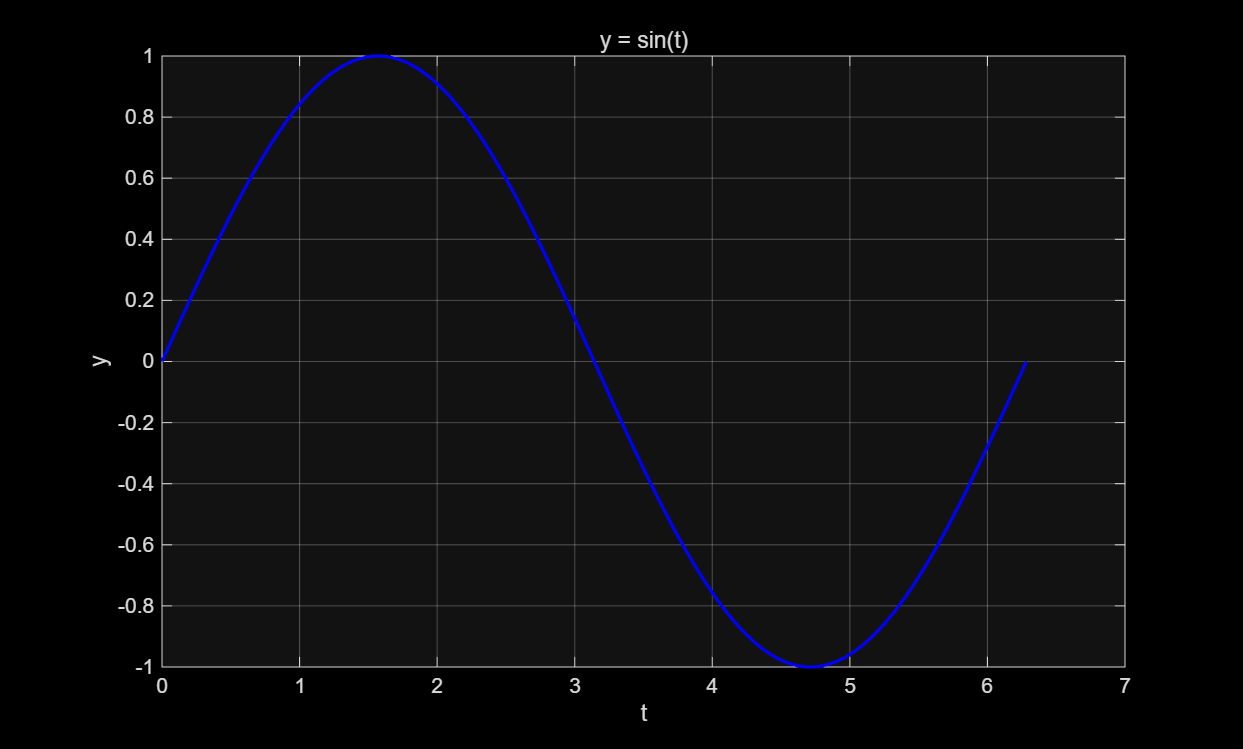
\includegraphics[width=0.48\textwidth]{./figures/Ex3_Task01_Figure_01.png}
    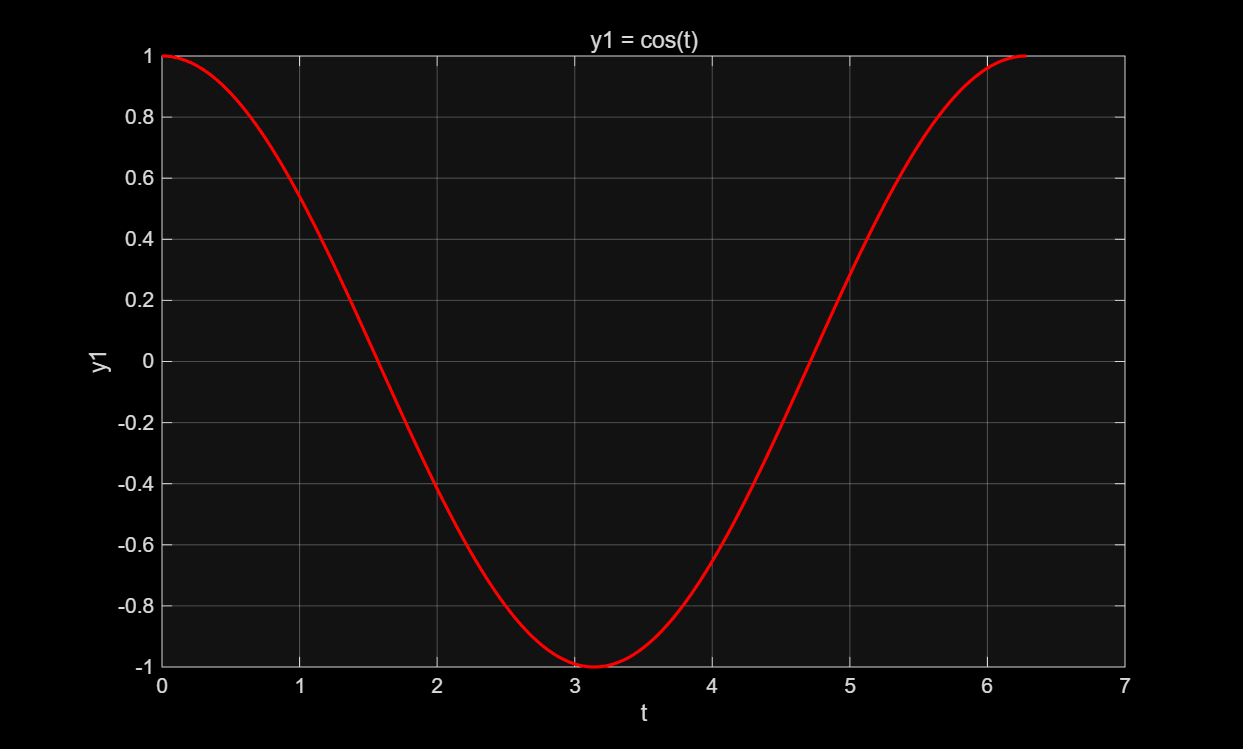
\includegraphics[width=0.48\textwidth]{./figures/Ex3_Task01_Figure_02.png}
    \caption{实验三 Task 01：Figure 1 ($y=\sin t$) 与 Figure 10 ($y=\cos t$)}
    \label{fig:ex3_task1}
\end{figure}

\textbf{实验结果：}
\begin{itemize}
    \item 根屏幕句柄值为0，其\texttt{ScreenSize}为$[1, 1, 1200, 800]$，\texttt{ScreenDepth}为32位
    \item Figure 1和Figure 10各自拥有独立的\texttt{CurrentAxes}句柄属性
    \item 图形窗口句柄为整数编号，根屏幕句柄为0（特殊值）
\end{itemize}

\subsubsection{Task 02：句柄层次结构探索}
通过\texttt{h.Children}、\texttt{gcf}、\texttt{gca}等命令探索图形对象之间的父子层次关系，并验证当前图形窗口切换时句柄值的变化。

\begin{figure}[H]
    \centering
    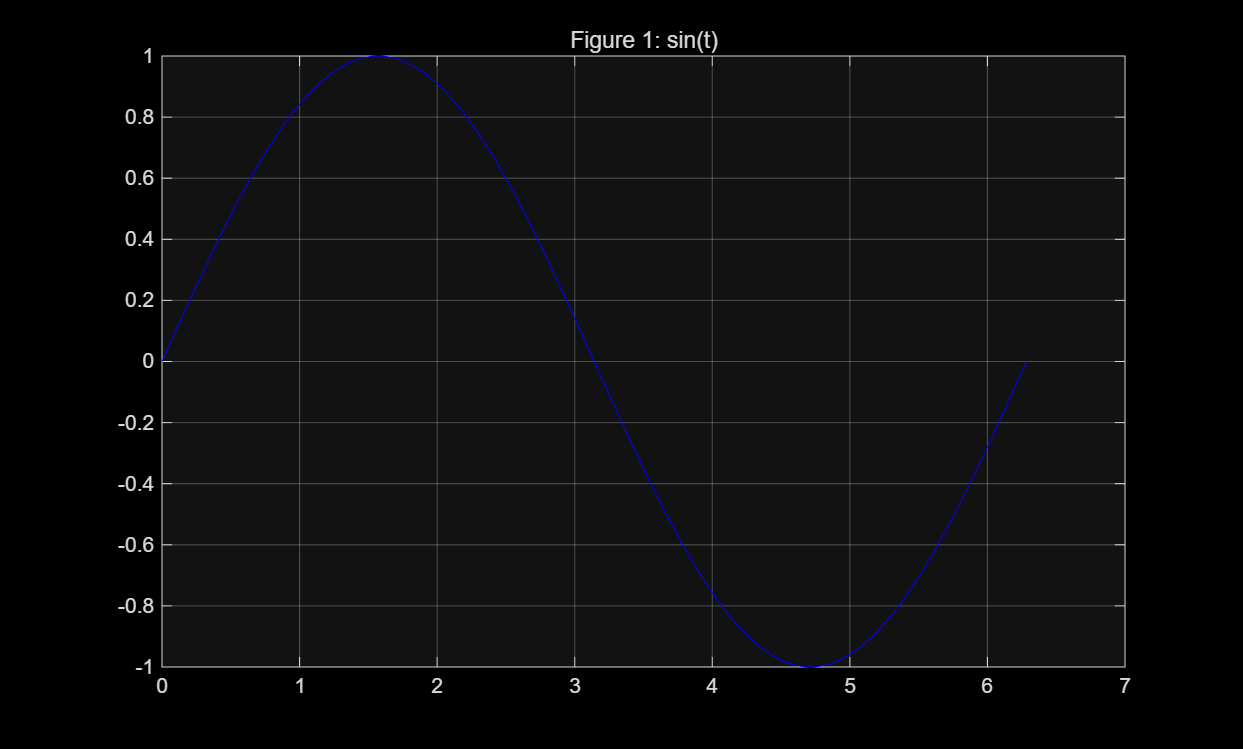
\includegraphics[width=0.48\textwidth]{./figures/Ex3_Task02_Figure_01.png}
    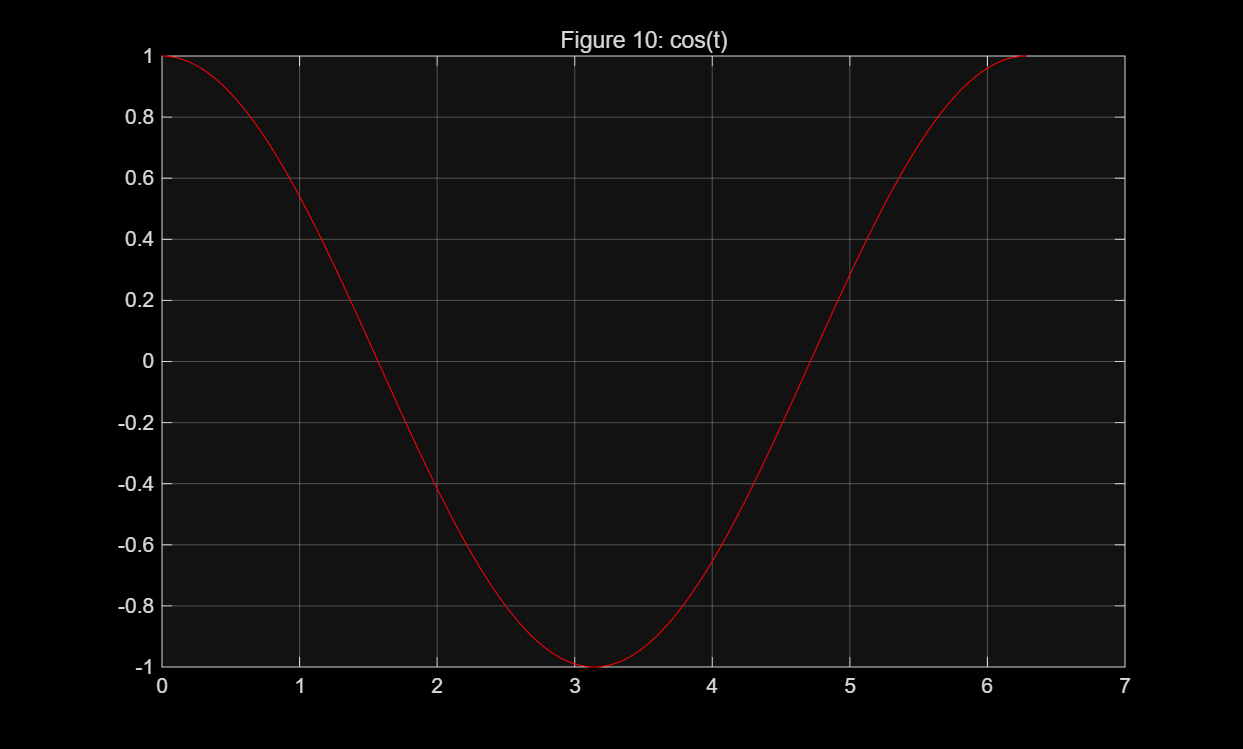
\includegraphics[width=0.48\textwidth]{./figures/Ex3_Task02_Figure_02.png}
    \caption{实验三 Task 02：句柄层次关系示意}
    \label{fig:ex3_task2}
\end{figure}

\textbf{实验结果：}
\begin{itemize}
    \item \texttt{h.Children}列出所有打开的图形窗口（Figure 10和Figure 1），按创建顺序倒序排列
    \item 调用\texttt{figure(1)}后，\texttt{gcf}的值从10变为1，证明当前图形窗口已切换
    \item \texttt{h1.Children}返回Figure 1的子对象（Axes句柄），\texttt{h2.Children}返回Figure 10的子对象
    \item \texttt{gca}始终指向当前活跃图形的Axes对象，随\texttt{gcf}切换而改变
\end{itemize}

\subsubsection{Task 03：图形属性设置与轴控制}
使用\texttt{set}函数修改图形对象的属性（如背景色、线条颜色），使用\texttt{axes()}函数将后续绘图定向到指定的坐标轴。

\begin{figure}[H]
    \centering
    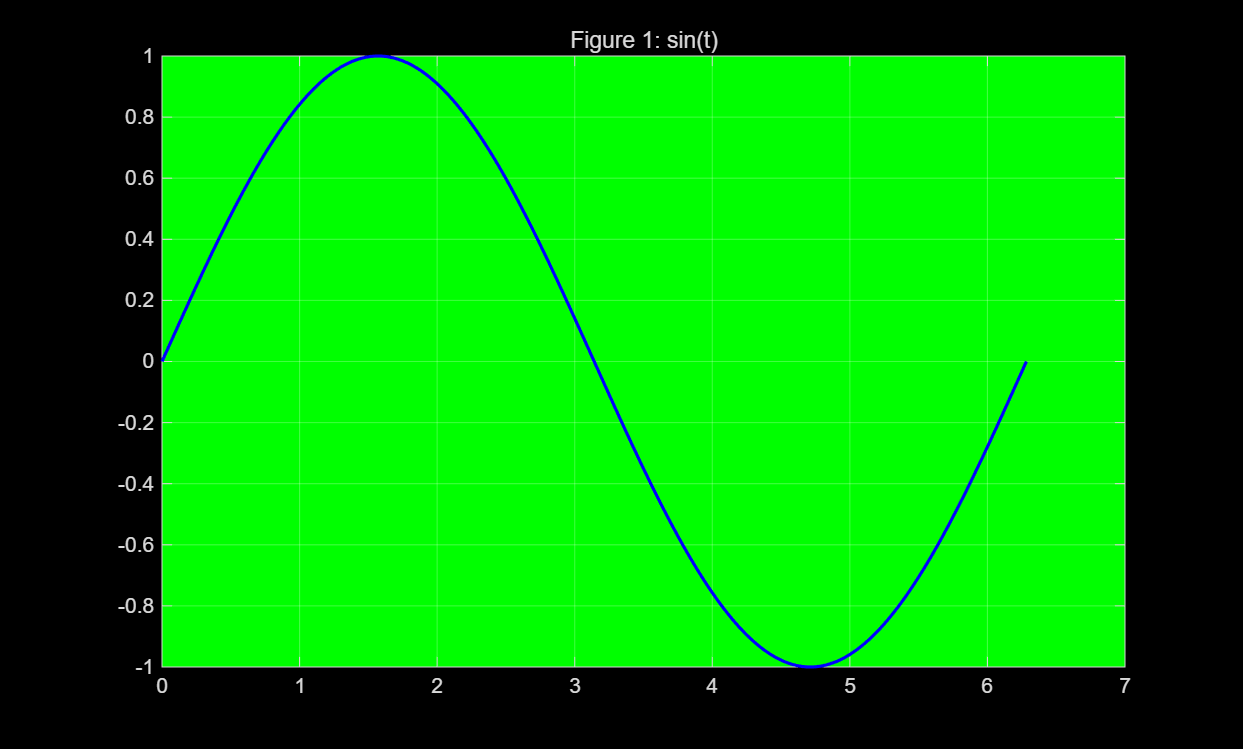
\includegraphics[width=0.48\textwidth]{./figures/Ex3_Task03_Figure_01.png}
    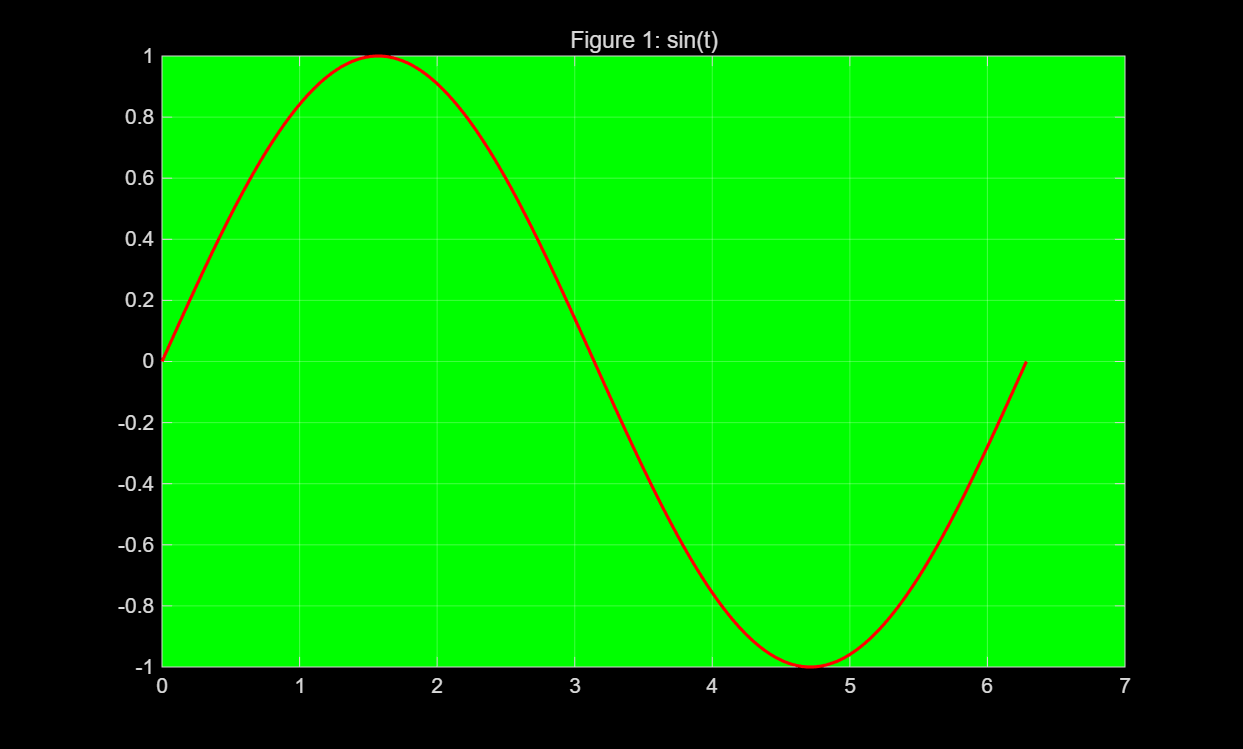
\includegraphics[width=0.48\textwidth]{./figures/Ex3_Task03_Figure_02.png}
    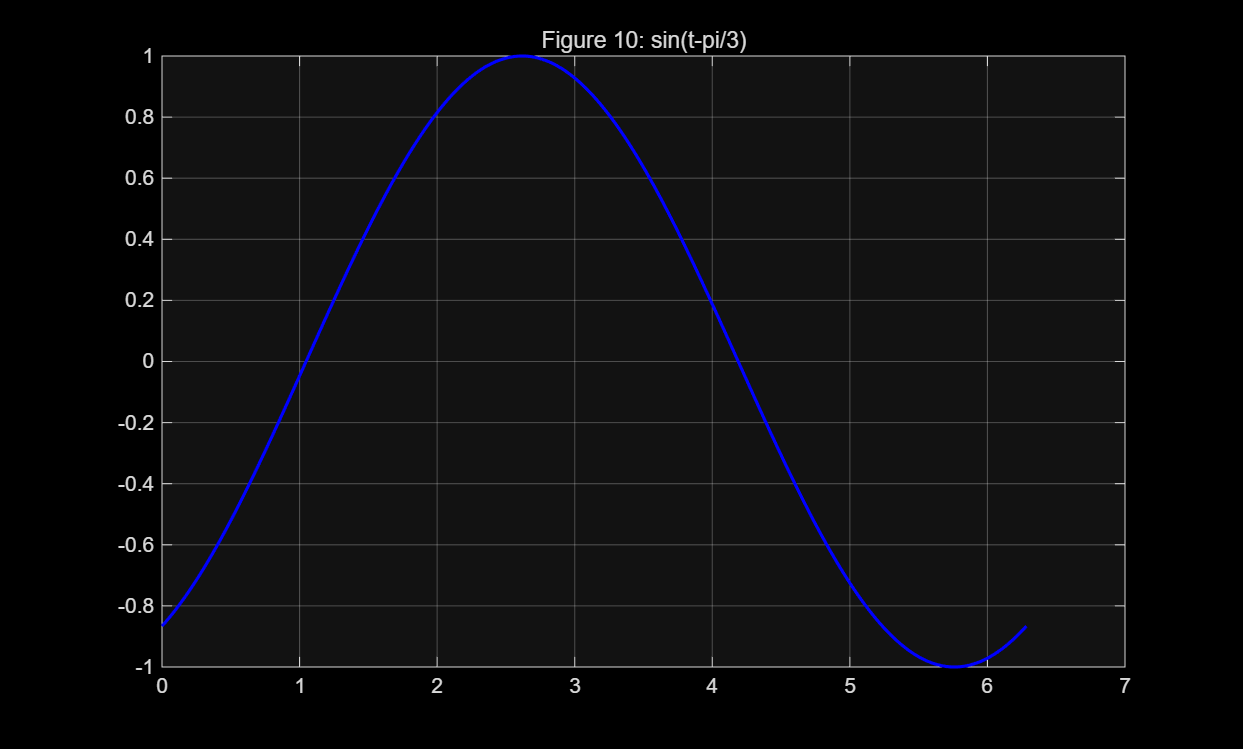
\includegraphics[width=0.48\textwidth]{./figures/Ex3_Task03_Figure_03.png}
    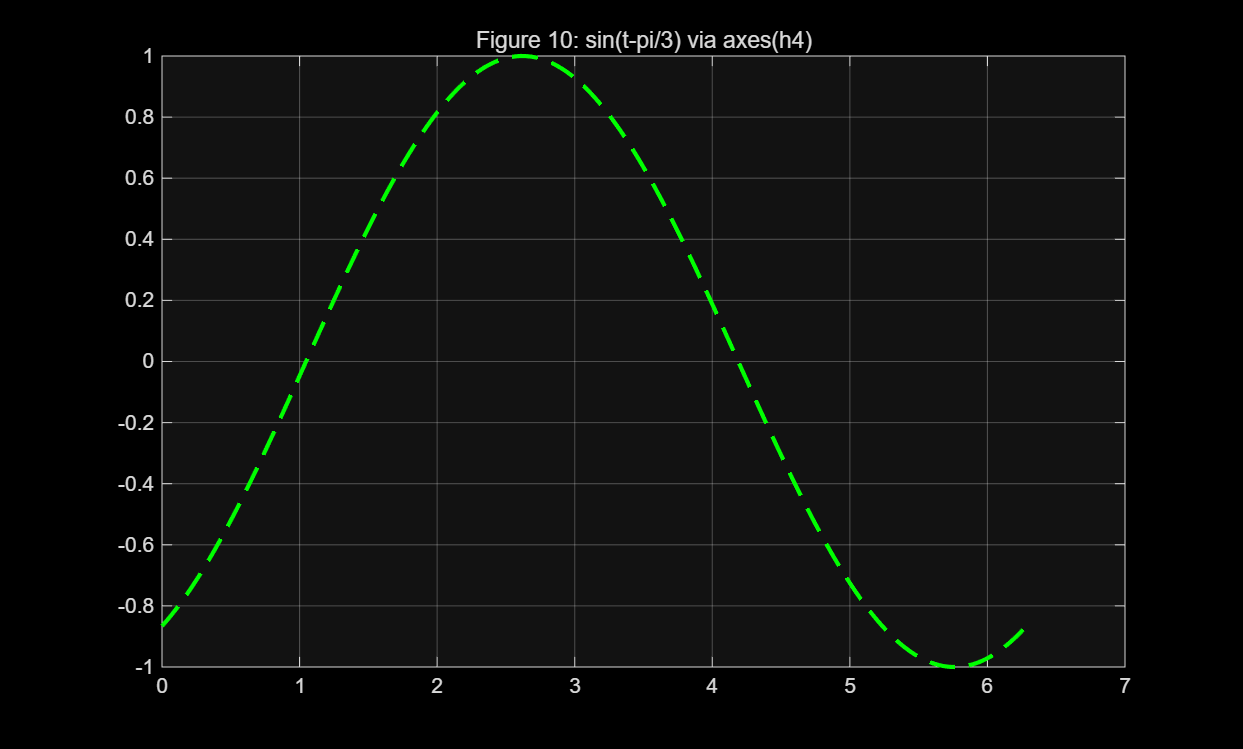
\includegraphics[width=0.48\textwidth]{./figures/Ex3_Task03_Figure_04.png}
    \caption{实验三 Task 03：属性设置效果对比 --- (左上) 绿色背景; (右上) 红色线条; (左下) 直接绘制; (右下) 通过axes(h4)定向绘制}
    \label{fig:ex3_task3}
\end{figure}

\textbf{实验结果：}
\begin{itemize}
    \item \texttt{set(h3, 'Color', 'green')}成功将Figure 1的坐标轴背景色改为绿色
    \item \texttt{set(h3\_1, 'Color', 'red')}成功将坐标轴中线条颜色改为红色
    \item \texttt{axes(h4)}可将后续\texttt{plot}命令的输出定向到指定的Axes对象h4（Figure 10的坐标轴），实现跨窗口绘图控制
\end{itemize}

\subsubsection{Task 04：控制系统分析GUI界面（高级编程）}
编写图形用户界面（GUI），实现对传递函数$G(s) = \frac{1}{s^2 + 2s + 1}$的Bode图、阶跃响应和Nyquist图分析功能。使用\texttt{uicontrol}创建按钮控件，回调函数调用控制系统工具箱中的\texttt{bode}、\texttt{step}、\texttt{nyquist}命令。

\begin{figure}[H]
    \centering
    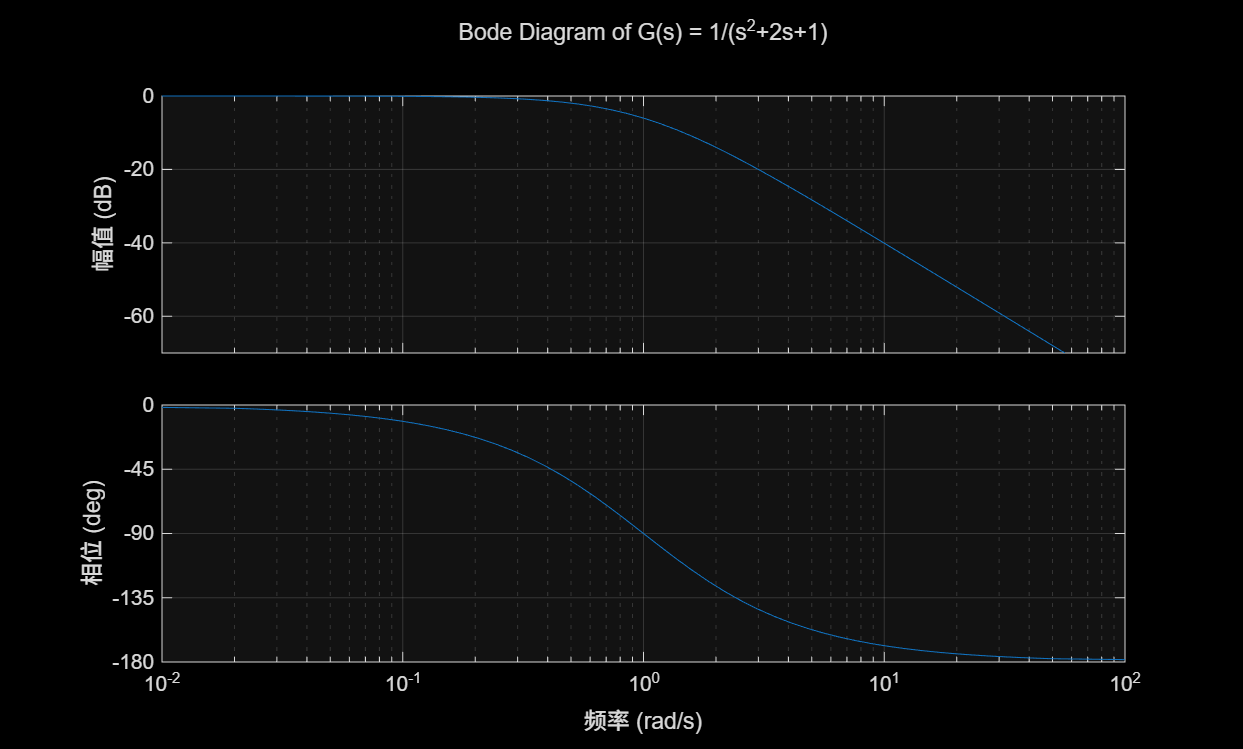
\includegraphics[width=0.48\textwidth]{./figures/Ex3_Task04_Figure_01.png}
    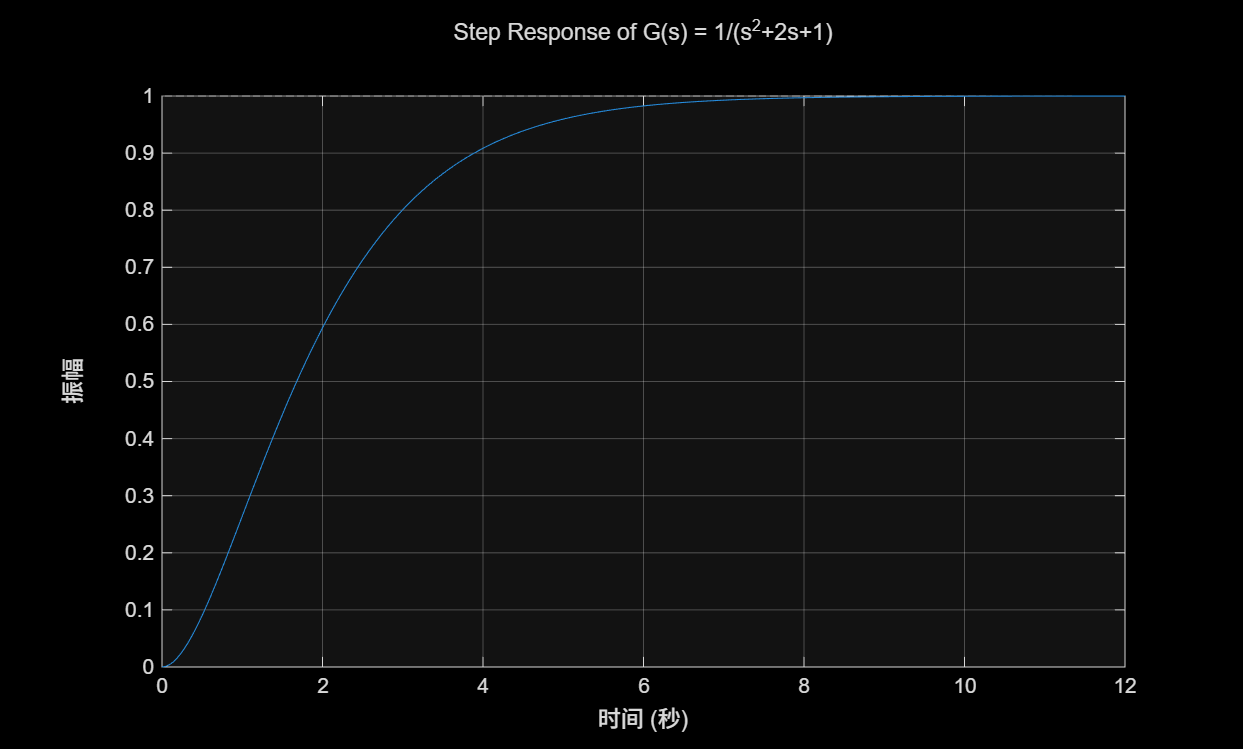
\includegraphics[width=0.48\textwidth]{./figures/Ex3_Task04_Figure_02.png}
    \caption{实验三 Task 04：Bode图与阶跃响应}
    \label{fig:ex3_task4a}
\end{figure}

\begin{figure}[H]
    \centering
    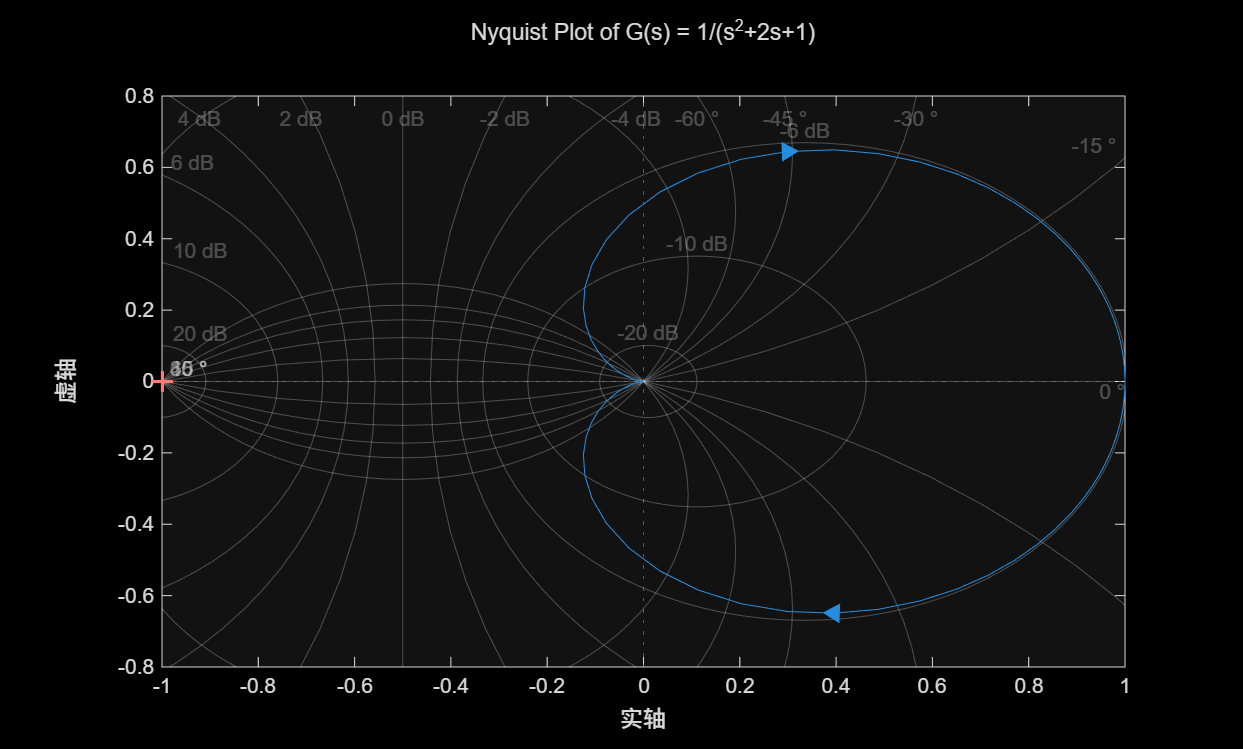
\includegraphics[width=0.65\textwidth]{./figures/Ex3_Task04_Figure_03.png}
    \caption{实验三 Task 04：Nyquist图}
    \label{fig:ex3_task4b}
\end{figure}

\textbf{实验结果：}成功创建了包含三个分析按钮的GUI界面，可分别调用Bode图、阶跃响应和Nyquist图分析功能。传递函数$G(s) = 1/(s^2 + 2s + 1) = 1/(s+1)^2$为临界阻尼二阶系统（$\zeta = 1$），Bode图显示幅频特性在$\omega = 1$ rad/s处转折，阶跃响应为单调上升无超调的临界阻尼响应。

\section{实验总结}
本次三个实验系统地学习了MATLAB在控制工程领域的基础应用，涵盖数值计算、程序设计、图形控制三个层面，为后续控制系统仿真实验奠定了坚实基础。

\subsection{实验一总结（MATLAB基本操作）}
\begin{enumerate}
    \item 掌握了MATLAB矩阵的输入、乘法运算、子矩阵提取及工作空间管理。注意矩阵乘法要求内维一致（A的列数 = B的行数）。
    \item 通过$y = \sin(1/t)$的绘制，理解了如何选择合适的采样步距来刻画函数的局部特征，特别是奇点附近需要更高的采样密度。
    \item 通过四个矩阵的属性分析，掌握了行列式（\texttt{det}）、秩（\texttt{rank}）、特征多项式（\texttt{poly}）、范数（\texttt{norm}）、特征值与特征向量（\texttt{eig}）、逆矩阵（\texttt{inv}）的计算，并观察了奇异矩阵（矩阵C）的特殊性质。
    \item 使用反斜杠运算符\texttt{\textbackslash}求解线性方程组，验证残差在机器精度范围内（$\sim 10^{-15}$），证明了MATLAB数值计算的可靠性和精度。
    \item 明确了矩阵运算（\texttt{*}, \texttt{/}, \texttt{\^}）与逐元素运算（\texttt{.*}, \texttt{./}）的本质区别。
    \item 掌握了在同一坐标系中使用\texttt{hold on}叠加多条曲线、用不同颜色和线型区分、以及通过\texttt{axis equal}控制坐标轴比例。
\end{enumerate}

\subsection{实验二总结（MATLAB编程）}
\begin{enumerate}
    \item 实现了for循环、while循环、向量化三种方式求和$2^i$，全部得到精确结果。向量化方法利用数学公式将计算复杂度从O(n)降至O(1)，体现了MATLAB向量化编程的优势。\texttt{uint64}类型对于大整数计算至关重要。
    \item 通过while循环找到了满足条件$1+2+\cdots+n < 10000$的最大n值（n=140），并用等差数列求和公式进行了验证。
    \item 编写了分段函数\texttt{ff.m}并验证了三个关键测试点，函数在$|x| \leq D$区间为线性，超出$\pm D$后饱和至$\pm h$，呈现限幅放大器特性。
\end{enumerate}

\subsection{实验三总结（MATLAB底层图形控制）}
\begin{enumerate}
    \item 理解了MATLAB图形对象的树形层次结构：Root $\to$ Figure $\to$ Axes $\to$ Lines/Text/Patches等。通过\texttt{Children}属性可遍历对象的子代。
    \item 掌握了\texttt{gcf}（当前图形窗口句柄）和\texttt{gca}（当前坐标轴句柄）的使用。\texttt{gcf}会随用户交互或\texttt{figure(n)}调用而改变，指向最近激活的图形窗口。
    \item 学会了使用\texttt{get}读取对象属性和\texttt{set}修改对象属性（如背景色、线条颜色）。\texttt{axes(handle)}可将后续绘图定向到指定的坐标轴对象。
    \item 通过GUI编程实践，掌握了\texttt{uicontrol}创建按钮等界面元素的方法，以及使用回调函数绑定控制逻辑。成功实现了传递函数$G(s)=1/(s^2+2s+1)$的Bode图、阶跃响应和Nyquist图分析。
\end{enumerate}

\section{实验源码}
以下列出三个实验的核心源代码（完整代码见附件目录Ex1/、Ex2/、Ex3/）。

\subsection{实验一核心源码}
\subsubsection{Task 01：矩阵输入与乘法}
\begin{lstlisting}[language=Matlab]
A = [1, 2, 3, 3; 2, 3, 5, 7; 1, 3, 5, 7; 3, 2, 3, 9; 1, 8, 9, 4];
B = [1+4i, 4, 3, 6, 7, 8; 2, 3, 3, 5, 5, 4+2i;
     2, 6+7i, 5, 3, 4, 2; 1, 8, 9, 5, 4, 3];
C = A * B;
D = C(end-1:end, end-2:end);
whos;
\end{lstlisting}

\subsubsection{Task 03：矩阵分析核心代码}
\begin{lstlisting}[language=Matlab]
detM = det(M);
fprintf('Rank: %d\n', rank(M));
fprintf('Characteristic polynomial: '); fprintf('%g ', poly(M));
fprintf('Norms: 1-norm=%g, 2-norm=%g, inf-norm=%g\n', norm(M,1), norm(M,2), norm(M,inf));
eigenvalues = eig(M);
[V, ~] = eig(M);  % V contains eigenvectors
if abs(detM) > 1e-12, invM = inv(M); else, fprintf('Singular.\n'); end
\end{lstlisting}

\subsubsection{Task 06：同一坐标系绘图}
\begin{lstlisting}[language=Matlab]
t = linspace(0, 2*pi, 2048);
plot(t, cos(t-0.5), 'r-', 'LineWidth', 1.5); hold on;
plot(t, sin(t-0.5), 'b--', 'LineWidth', 1.5); hold off;
xlabel('t'); ylabel('y');
legend('cos(t-0.5)', 'sin(t-0.5)'); grid on; axis equal;
\end{lstlisting}

\subsection{实验二核心源码}
\subsubsection{Task 01：2的幂次求和（向量化方法）}
\begin{lstlisting}[language=Matlab]
% for loop
sumFor = uint64(0); term = uint64(1);
for i = 0:63, sumFor = sumFor + term; term = bitshift(term, 1); end

% while loop
sumWhile = uint64(0); term = uint64(1); i = 0;
while i <= 63, sumWhile = sumWhile + term; term = bitshift(term, 1); i = i + 1; end

% Vectorized: geometric series formula
sumVectorized = uint64(2^64 - 1);
\end{lstlisting}

\subsubsection{Task 03：分段函数ff.m}
\begin{lstlisting}[language=Matlab]
function y = ff(x)
    D = 1; h = 10;
    if x > D, y = h;
    elseif abs(x) <= D, y = (h/D) * x;
    else, y = -h;
    end
end
\end{lstlisting}

\subsection{实验三核心源码}
\subsubsection{Task 02：句柄层次探索}
\begin{lstlisting}[language=Matlab]
h = get(0);          % Root screen
h.Children           % All open figure windows
figure(1); gcf;      % gcf = 1 after switching
h1.Children;         % Axes of Figure 1
h2.Children;         % Axes of Figure 10
gca;                 % Current axes
\end{lstlisting}

\subsubsection{Task 03：属性设置}
\begin{lstlisting}[language=Matlab]
h3 = h1.Children;                      % Get Axes of Figure 1
set(h3, 'Color', 'green');             % Set background color
h3_1 = get(h3, 'Children');            % Get Line child of Axes
set(h3_1, 'Color', 'red');             % Set line color
h4 = h2.Children; axes(h4);            % Direct subsequent plots to h4
plot(t, sin(t - pi/3));
\end{lstlisting}

\subsubsection{Task 04：控制系统分析}
\begin{lstlisting}[language=Matlab]
sys = tf(1, [1, 2, 1]);    % G(s) = 1/(s^2+2s+1)
bode(sys); grid on;         % Bode plot
step(sys); grid on;         % Step response
nyquist(sys); grid on;      % Nyquist plot
\end{lstlisting}

\end{document}
